\documentclass[a4paper,12pt]{article}
% Resten af pakkerne
\usepackage[english, danish]{babel}
\usepackage{csquotes}
\usepackage{float}
\usepackage{flafter}
\usepackage{graphicx}
\usepackage{setspace}
\usepackage{enumitem}
\usepackage{multirow}
\usepackage{lmodern}
\usepackage{amssymb,amsmath}
\usepackage{ifxetex,ifluatex}
\usepackage{lastpage} % Bruges i customtitlepage til at tælle sider
\usepackage[font=small,labelfont=bf]{caption}
\usepackage{lscape}
\usepackage{xargs}
\usepackage{tabularx}

\usepackage{ifthen}

\usepackage{xcolor}
% \usepackage{csvsimple}
\usepackage{longtable}

% Margin
\usepackage{geometry}
\geometry{a4paper,  total={170mm,250mm},
 left=20mm,
 top=30mm}


% New Commands
\newcommand\myworries[1]{\textcolor{red}{#1}} 
\newcommand{\myparagraph}[1]{\paragraph{#1}\mbox{}\\}


% Needs to be the last package included
\usepackage{hyperref}
\hypersetup{
    colorlinks=true,
    linkcolor=black,
    filecolor=magenta,      
    urlcolor=blue,
    citecolor=black,
}


% Linjemellemrum
% \linespread{1.4}
\graphicspath{{./figures/}{../figures/}}

\begin{document}
% Fjerner side tal
\pagenumbering{gobble}
    \renewcommand{\thesection}{\Roman{section}} 
    \renewcommand{\thesubsection}{\thesection.\Roman{subsection}}
    % Forside
    \begin{titlepage}
\begin{center}
% Title
{ \LARGE \bfseries Creditoro \\[0.4cm]}
Et krediteringssystem
\begin{figure}[H]
\centering 
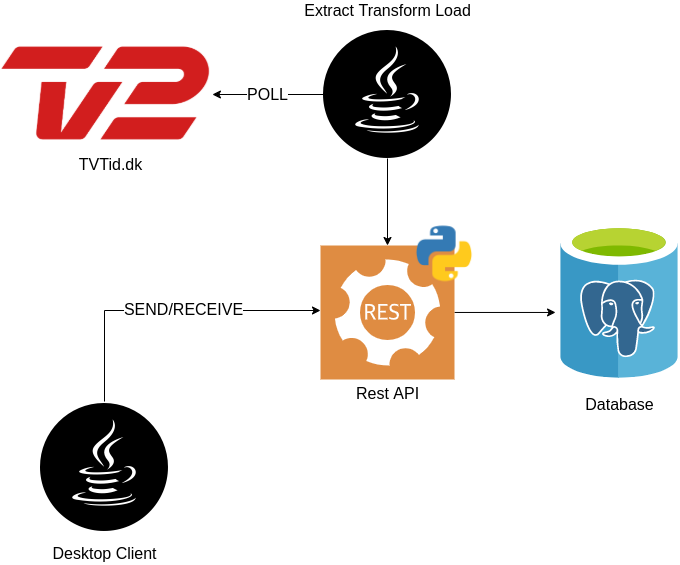
\includegraphics[scale=0.5]{figures/creditoro.png}
\label{figure:creditoro_system}
\end{figure}

Softwareteknologi\\
\vspace{2mm}
Semesterprojekt 2. semester, ST2-PRO\\
\vspace{2mm}
\textbf{Projektperiode:} 01.01.2020 - 29.05.2020 \\
\vspace{2mm}
\textbf{Afleveringsdato:} 29.05.2020 \\

\vspace{7mm}

\textbf{Projektgruppe 06:} \\
\vspace{2mm}
Jakob Rasmussen, jakra19@student.sdu.dk \\
\vspace{2mm}
Kenneth M. Christiansen kechr19@student.sdu.dk \\
\vspace{2mm}
Kevin K. M. Petersen, kepet19@student.sdu.dk \\
\vspace{2mm}
Kristian N. Jakobsen, kjako19@student.sdu.dk \\
\vspace{2mm}
Mathias N. Rasmussen, mara816@student.sdu.dk \\
\vspace{2mm}
Simon Jørgensen, sijo819@student.sdu.dk \\

\vspace{7mm}

\textbf{Vejleder:} Henrik Lykkegaard Larsen, hlla@mmmi.sdu.dk \\

% Bottom of page
\vfill

Syddansk Universitet\\
Det Tekniske Fakultet\\
Mærks Mc-Kinney Møller Instituttet\\
Campusvej 55, 5230 Odense M

\end{center}
\end{titlepage}
    \newpage
    
    % Titelblad 
    \begin{tabular}{@{}l l} 
\textbf{Title:} & Creditoro \\
& \\
\textbf{Institution:} & Syddansk Universitet \\
& Det Tekniske Fakultet, Mærsk Mc-Kinney Møller Instituttet \\
& Campusvej 55, 5230 Odense M \\
& \\
\textbf{Uddannelse:} & Softwareteknologi \\
& \\
\textbf{Semester:} & 2. Semester \\
& \\
\textbf{Semestertema:} & Udvikling af cyber-physical softwaresystemer \\
& \\
\textbf{Kursuskode:} & ST2-PRO \\
& \\
\textbf{Projektperiode:} &  01.01.2020 - 29.05.2020\\
& \\
\textbf{ECTS:} & 10 ECTS\\
& \\
\textbf{Vejleder:} & Henrik Lykkegaard Larsen\\
& \\
\textbf{Projektgruppe:} & 06\\
& \\

\\
\end{tabular}

% VARIABLES
\newcounter{PROD}
\setcounter{PROD} {0}

%%%%


% Jakob Jakob Jakob Jakob Jakob Jakob Jakob Jakob Jakob Jakob Jakob
\ifnum \value{PROD}=1
    
\includegraphics[scale=0.07]{figures/signatures/signatureJR.jpg}
    \vspace{-9.5mm}
\fi
\par\rule{\textwidth}{0.4pt}

Jakob Rasmussen, jakra19@student.sdu.dk\\
% -end- -end- -end -end -end- -end- -end -end -end- -end- -end -end -end-

% Kenneth Kenneth Kenneth Kenneth Kenneth Kenneth Kenneth Kenneth Kenneth

\ifnum \value{PROD}=1
    
\includegraphics[scale=0.3]{figures/signatures/signature_kechr19.PNG}
    \vspace{-5mm}
\fi
\par\rule{\textwidth}{0.4pt}

Kenneth M. Christiansen, kechr19@student.sdu.dk\\
\vspace{3.5mm}
% -end- -end- -end -end -end- -end- -end -end -end- -end- -end -end -end-

% KEVIN KEVIN KEVIN KEVIN KEVIN KEVIN Kevin Kevin Kevin Kevin Kevin Kevin
\vspace{-6.5mm}

\ifnum \value{PROD}=1
    
\includegraphics[scale=0.3]{figures/signatures/signature_kepet19.png}
    \vspace{-8mm}
\fi
\par\rule{\textwidth}{0.4pt}

Kevin K. M. Petersen, kepet19@student.sdu.dk
% -end- -end- -end -end -end- -end- -end -end -end- -end- -end -end -end-

% Kristian Kristian Kristian Kristian Kristian Kristian Kristian

\ifnum \value{PROD}=1
    
\includegraphics[scale=0.04]{figures/signatures/signature_kjako19.jpg}
    \vspace{-9.5mm}
\fi
\par\rule{\textwidth}{0.4pt}

Kristian N. Jakobsen, kjako19@student.sdu.dk\\
% -end- -end- -end -end -end- -end- -end -end -end- -end- -end -end -end-

% Mathias Mathias Mathias Mathias Mathias Mathias Mathias Mathias Mathias

\ifnum \value{PROD}=1
    
\includegraphics[scale=0.120]{figures/signatures/Signatur_mara816.png}
    \vspace{-5mm}
\fi
\par\rule{\textwidth}{0.4pt}

Mathias N. Rasmussen, mara816@student.sdu.dk\\
% -end- -end- -end -end -end- -end- -end -end -end- -end- -end -end -end-

% Simon Simon Simon Simon Simon Simon Simon Simon Simon Simon Simon Simon

\ifnum\value{PROD}=1
    
\includegraphics[scale=0.042]{figures/signatures/signatureSJ.png}
    \vspace{-3.5mm}
\fi
\par\rule{\textwidth}{0.4pt}

Simon Jørgensen, sijo819@student.sdu.dk\\
% -end- -end- -end -end -end- -end- -end -end -end- -end- -end -end -end-


%Bottom of page
%\vfill


\begin{tabular}{@{}l l}
Antal sider:    & \myworries{sider} \\ % \pageref{LastPage} virker ikke mere, da der ikke er sidetal på bilag
Bilag:          & 1 bilag 
\end{tabular}

\vspace{3.5mm}

\begin{footnotesize}

\textbf{Ved at underskrive dette dokument bekræfter hvert enkelt gruppemedlem, at alle
har deltaget lige i projektarbejdet, og at alle således hæfter kollektivt for rapportens indhold.}
\end{footnotesize}
    \newpage

    % Resume
    \section{Resume}
Denne sektion skal indeholde:

\begin{itemize}
    \item Hovedresultater og konklusioner  – hvad kom der ud af arbejdet
\end{itemize}{}

I dette projekt bliver der arbejdet ud fra TV2's problemstilling omhandlende muligheden for at flytte krediteringer fra TV til en anden platform. \myworries{Denne plads kan så udfyldes med andet som fx. reklamer og promoveringer for egne programmer.} Gruppen har valgt at bygge et fuldt funktionelt program, inklusive Rest API og EPG poller. Dertil er gruppen fundet frem til en problemformulering der omhandler udviklingen af et krediteringssystem, hvordan krediteringerne skal gøres tilgængelige samt håndteres. Derudover undersøges det hvordan systemet kan indeholde krediteringerne.
Projektgruppen har valgt at afgrænse projektet ved at lave en prototype til et færdigt program. Ideelt ville systemet også have en webside, dog er dette vurderet til værende udenfor projektets scope.

Overordnet benyttes UP (Unified Process) i hele projektet. UP opdeler hele projektet i 4 faser: \textit{Inceptionsfasen} hvor vigtige krav og kristiske risici identificeres. \textit{Elaborationfasen} hvor en iterativ udvikling af krav, design, analyse og test konstrueres ud fra overordnede kravspecifikationer. \textit{Konstruktionfasen} hvor systemet konstrueres - den faktiske kodeudformning. \textit{Overgangsfasen} hvor det undersøges om systemet er færdigt og ikke har mangler.

I starten af projektets analysefase er et brugsmønsterdiagram, herunder aktørliste og brugs-mønsterliste, udformet. Dette er med til at give et billede af hvordan systemet skal bygges op, samt hvilke aktører der skal kunne interagere med hvilke brugsmønstre. Til prioritering af brugsmønstrene er der foretaget en MoSCoW-analyse.
Til identificering af ikke-funktionelle krav er der brugt metoden FURPS. Her er der sat krav op der omhandler Functionality, Usability, Reliability, Performance og Supportability. For yderligere specificering af ikke funktionelle krav er FURPS+ benyttet - FURPS med ekstra specificerende kategorier med til at opfylde kundens behov.

Til projektstyring benyttes Scrum til at fordele og få overblik over de forskellige opgaver, der opdeles i mindre issues. De forskellige arbejdsopgaver inddeles i sprints som forløber sig over en given periode - i dette projekts tilfælde to uger.

\myworries{Hovedresultater og konklusioner}



    \newpage
    
    % Forord
    \section{Forord}
Denne sektion skal indeholde:

\begin{itemize}
    \item Hensigten med rapporten, målgruppe, forhistorie, anerkendelser
\end{itemize}{}

    \newpage

    % Indholdsfortegnelse
    \setcounter{tocdepth}{2} % anything below subsection will not be added
    \tableofcontents
    \newpage
    
    % Læsevejledning
    \input{tex/vi_læsevejledning}
    \newpage
    
    \section{Redaktionelt}

    \newpage
    
    % Start counting from this line
    \pagenumbering{arabic}
    \setcounter{page}{1}

    \renewcommand{\thesection}{\arabic{section}} 
    \renewcommand{\thesubsection}{\thesection.\arabic{subsection}}
    \setcounter{section}{0}
    % Introduktion
    \section{Indledning}

\myworries{Formål og mål med projektet.}\\

% ------------------------ Baggrund for projektet ------------------------------------------------
Når et program bliver broadcasted på en TV station skal krediteringer vises. Dette gøres i slutningen af programmet, i maksimalt 30 sekunder. Det betyder, at der ikke altid er tid til at vise alle krediteringer, og derfor prioriteres de før de vises. \\
Hvis de 30 sekunder for hvert program kunne frigøres, kan danske TV stationer bruge tiden på at vise noget andet, som f.eks. reklamer og promovering af eget indhold. Derved har TV 2 mulighed for at øge deres årlige indtægter med op til 60 millioner kroner. \\
TV 2 har brug for et system, der kan administrere krediteringer for programmer produceret i Danmark. Hertil skal der kunne tilføjes nye krediteringer i systemet for nye produktioner, samt det skal være muligt at kunne søge efter eksisterende krediteringer. Det skal være muligt at kunne se hvilken rolle en given person har haft i en produktion, da denne person kan have haft flere forskellige roller på flere forskellige produktioner.

% ------------------------ Projektets rammer og baggrunden for projektet -------------------------
\subsection{Projektrammer}
Denne sektion har til formål at opridse rammerne for projektet, samt hvilket område projektgruppen arbejder indenfor.

\subsubsection{Krav til Projektet}
Systemet skal så vidt muligt skrives i programmeringssproget Java. \\
Krediterings-data skal lagres i en database, og i dette projekt skal den brugte database være SQL baseret. Der skal bruges PostgreSQL.\\
Systemet forventes ikke at være et færdigt system, men en række forslag til løsninger der opfylder systembehovet. Forslagene skal inkludere:

% ------------------------- OPDATER DENNE TIDSPLAN ----------------------------------------------
\begin{itemize}
    \item Krav
    \item Analyse
    \item Design
    \item Implementering
    \item Test
\end{itemize}
% ----------------------------------------------------------------------------------------------

\noindent
Producere der kan tilføje og redigere i krediteringerne, skal kun have mulighed for at redigere i de produktioner, de selv ejer.\\
Det forventes at krediteringssystemet er kompatibelt med andre systemer (f.eks. fra Stofa, YouSee etc.).

\subsubsection{Tidsplan}
Tidsplanen har til formål at skabe overblik og styring over projektet. 
Den giver gruppemedlemmerne et overblik over, hvornår de forskellige dele af projektet skal starte og slutte, og derved bliver det hurtigt klart hvis tidsplanen skrider. \\

\begin{landscape}
    \begin{figure}
        \centering
        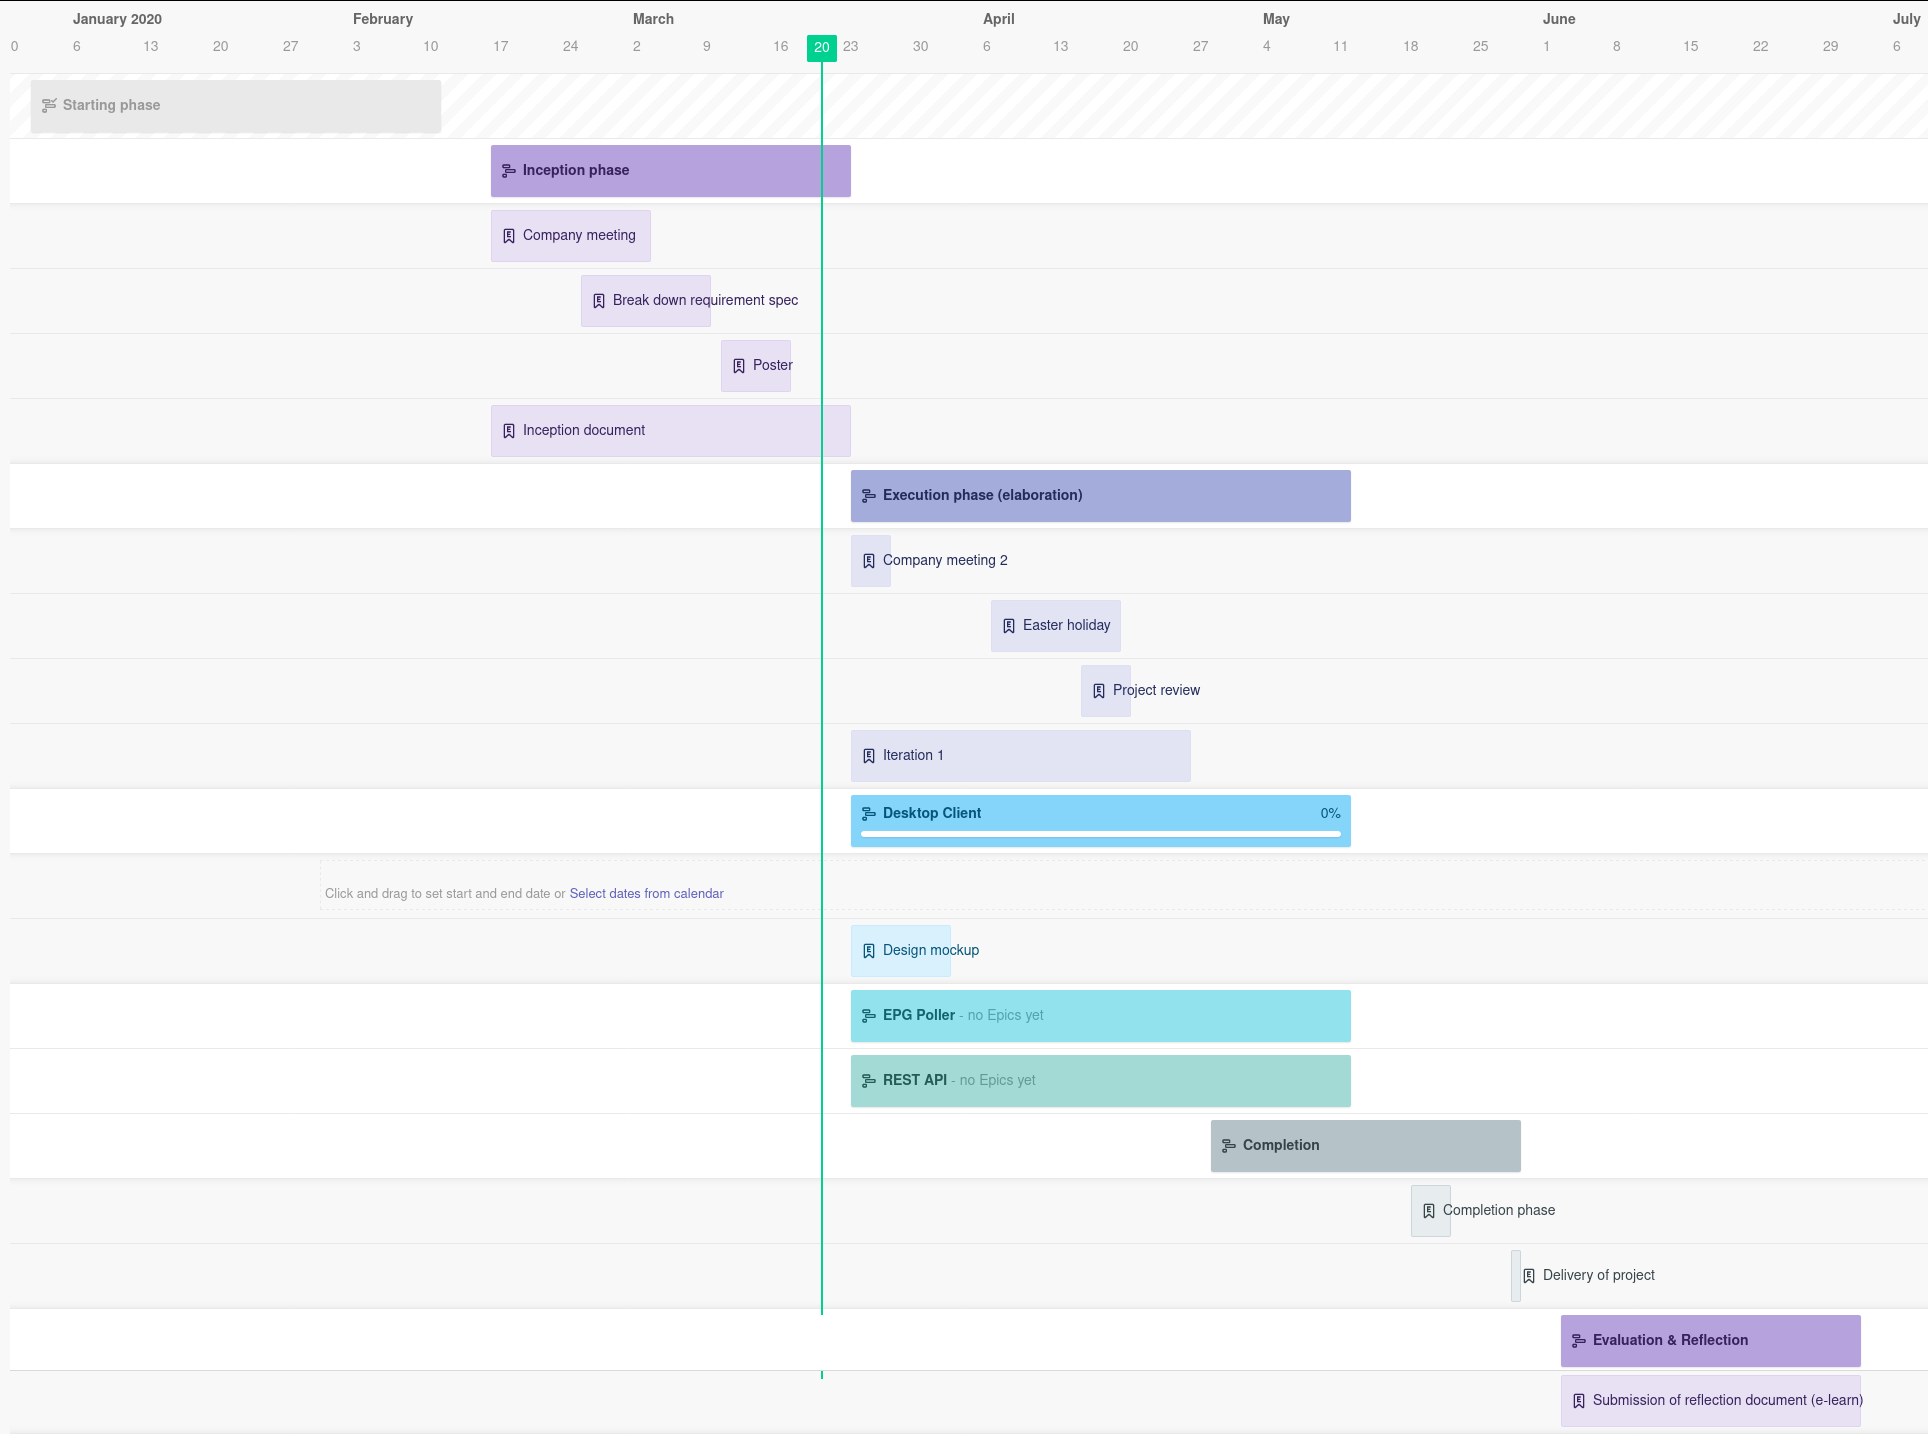
\includegraphics[scale=0.30]{figures/grantt_udvidet.png}
        \caption{Tidsplan for projektet}
        \label{fig:gantt}
    \end{figure}{}
\end{landscape}


% ------------------------ Resume af udleverede case ----------------------------------------------
\subsubsection{Igangsættende Problem}
TV2 ønsker at frigøre 30 sekunders krediterings tekster efter hvert program, så de i stedet kan bruge tiden på at vise reklamer. Problemet består i at disse krediterings tekster, så skal vises på en anden platform. I tabel \ref{table:kravFraCase} ses kravene fra TV2's projektcase: \\

\begin{table}[ht]
    \begin{tabularx}{\textwidth}{|p{10cm}|X|}
        \hline
        \textbf{Beskrivelse} & \textbf{Type} \\
        \hline
        “Vi har brug for  et krediterings system der kan  håndtere  dansk TV content” 
        & En vag opgave \\
        
        \hline
        "Dette inkluderer muligheden for at oprette nye krediteringer i systemet, når en ny produktion bliver lavet, samt at have mulighed for at søge efter en given produktion og få en liste af krediteringer, forbundet til denne. Det burde også være muligt at se hvilken rolle en given person har haft i en produktion, eftersom en person kan have flere forskellige roller i forskellige produktioner."
        & Ønske om en bestemt løsning \\
        
        \hline 
        "Producers/TV-stationer burde være i stand til at redigere krediteringer for programmer/produktioner de ejer. De burde også være i stand til at redigere disse produktioners ID. Systemadministratorer skal kunne vedligeholde (oprette, læse, opdatere og slette) personer, krediteringer og personer."
        & Ønske om en bestemt løsning \\
        
        \hline
        "Til slut skal systemet kunne offentliggøre en service som andre systemer kan bruge. Disse systemer kan f.eks. være en hjemmeside eller en applikation. Disse andre systemer skal også kunne bruge API'et, så data'et kan blive brugt i allerede eksisterende systemer (såsom TVTID.dk - TV 2's TV-Guide)."
        & Ønske om en bestemt løsning \\
        
        \hline
        "En form for adgangskontrol skal implementeres, til de beskyttede dele af systemet (oprettelse, opdatering, slettelse, osv. af data)
        & Ønske om en bestemt løsning \\
        
        \hline
        "Der skal være en offentligt tilgængelig del af systemet, hvor det er muligt at se krediteringer uden at logge ind."
        & Ønske om en bestemt løsning \\
        
        \hline
        “Nuværende løsning er begrænset til 30 sekunder, og dermed kan alle krediteringerne ikke altid vises i praksis” 
        & Et problem \\
        \hline
    \end{tabularx}    
    \caption{Krav fra TV2s projektcase}
    \label{table:kravFraCase}
\end{table}


% ------------------------- Identifikation af problemet -----------------------------------------------------
\subsubsection{Identifikation af Problemet}
Som det er nu bliver krediteringer vist i slutningen af et program. Ifølge reglerne for visning af krediteringer, må krediteringer ikke vises mere end 20 sekunder for produktioner under 60 minutter, og 30 sekunder for produktioner over 60 minutter. Dette giver en del problemer. For det første betyder den begrænsede varighed, at ikke alle medarbejdere kan krediteres. Dette ender ud i at der skal prioriteres i krediteringerne, før de bliver vist på TV. Derved får alle medarbejdere ikke den anerkendelse de burde.
Hvis krediteringer flyttes til et eksternt system, og derved ikke bliver vist på TV, kan man undgå at skulle prioritere. Alle kan derved få den fortjente kredit. Derudover vil det også give mulighed for at vise noget andet, som f.eks. reklamer eller promoveringer for eget indhold. \cite{DR-Krediteringsregler} \\

\noindent
Et sådan eksternt system vil også hjælpe med oprettelsen af nye krediteringer, ved at gøre processen hurtigere og nemmere, samt mere overskueligt. Dertil har gruppen valgt at arbejde med samtlige/alle problemstillinger givet af TV2 i tabel \ref{table:kravFraCase}, og lave en prototype til et funktionsdygtigt system. Angående valget med at arbejde med samtlige problemstillinger præsenteret af TV2, har gruppen konkluderet det som værende realistisk jævnfør figur \ref{fig:gantt}. Denne prototype vil kunne bruges som et udkast til et endeligt system.


% ------------------------- Formål med projektet -----------------------------------------------------
\subsection{Formål med Projektet}
Projektet har til formål at gøre gruppemedlemmerne i stand til at tilrettelægge og gennemføre udviklingen af en softwareapplikation i en agil udviklingsproces. Den udvilklingsproces der tages i brug i dette projekt, er Unified Proces. I tæt sammenspil med den agile udvilkingsmetode SCRUM, opnåes viden om, hvordan man går fra objektorienterede systemmodeller til implementering af kode. Ydermere er formålet, at gruppen opnår viden omkring databaser, og hvordan man udarbejder et databasedesign, laver databaseforespørgelesr og bruger disse i applikationen.


% ------------------------ Problemformulering & Afgrænsning ------------------------------------------
\subsection{Problemformulering \& Afgrænsning}
Ud fra overstående er projektgruppen er kommet frem til følgende problemformulering med tilhørende underspørgsmål:\\

\noindent
\textit{Hvordan kan vi udvikle et samlet krediteringssystem, der giver mulighed for at erstatte rulletekster efter et endt program?}

\begin{enumerate}
    \item Hvem skal kunne håndtere krediteringer?
    \item Hvordan skal krediteringerne gøres tilgængelige, og hvordan skal seerne refereres dertil?
    \item Hvordan kan man oprette et system som kan indeholde krediteringer?\\ % <- skal være der for at holde afstand til afgrænsningen
\end{enumerate}


% afgrænsning
\noindent 
Projektgruppen har valgt at afgrænse dette projekt, ved at konstruere en prototype til et system. Det er blevet valgt at lave et system der ligger tæt op ad det oprindelige foreslag fra TV2s projektcase, hvor systemtegningen kan ses på figur \ref{fig:tv2_system}, og et sådan system vil indebære alle kravene i tabel \ref{table:kravFraCase}.
\begin{figure}[H]
    \centering
    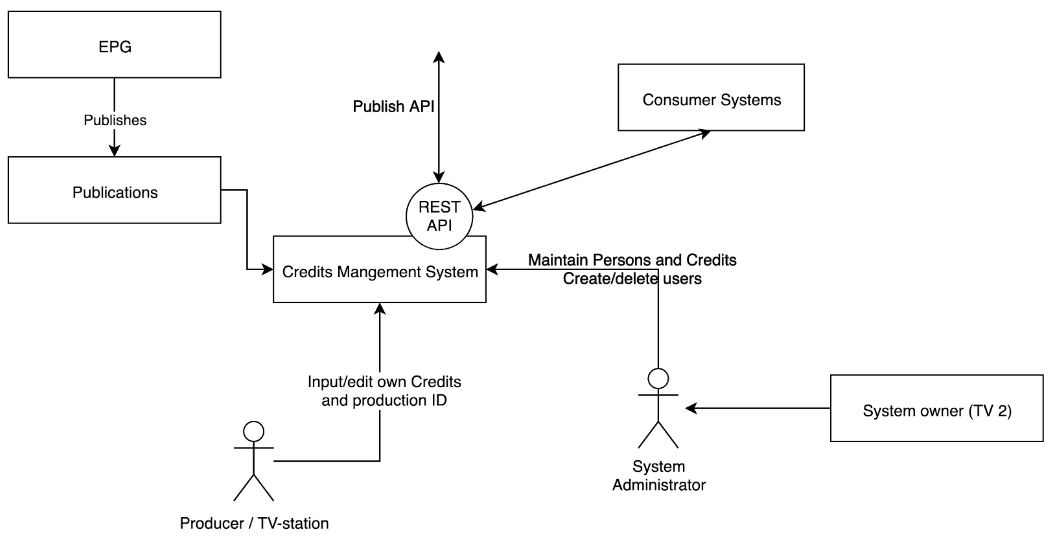
\includegraphics[scale=0.4]{figures/tv2_system.png}
    \caption{Foreslag til systemtegning - © TV2}
    \label{fig:tv2_system}
\end{figure}

\noindent % Det vi vælger fra:
I et produktionsklart system vil det være ideelt at have en webside, men dette har vi konkluderet som værende uden for projektet.
    \newpage
    
    % Metode & Planlægning
    \input{tex/2_metode_og_planlægning}
    \newpage
    
    % Faglige vidensgrundlag
    \section{Faglige Vidensgrundlag}
Dette afsnit har til formål at dække over den faglige viden gruppen skal have, for at kunne udføre projektet.

\subsection{JAVA}
At have kendskab til Java er en vigtig forudsætning for udarbejdelsen af projektet. Systemet vil hovedsageligt blive programmeret i sproget Java. Det faglige niveau svarer til 2. semesterstuderende på Softwareteknologi. Dette indebærer blandt andet forståelse af JavaFX og Scenebuilder.
Arbejdet med Java i projektet forudsætter derudover forståelse for basale programmeringsprincipper og forståelse for det objektorienterede programmeringsparadigme. 

\subsection{Python}
Et grundlæggende kendskab til Python kræves for at kunne forstå samt implementere REST Api'et.

\subsection{Database}
Systemet vil indeholde en lang række data, som skal lagres i en database. Det er derfor nødvendigt at have forståelse for databaser, databasestrukturer, relationelle SQL-databaser og SQL-queries. Databasen der vil blive benyttet i projektet er PostgreSQL, en basal viden om databasesproget/programmeringssproget SQL er derfor nødvendigt. 
Al nødvendig viden er givet i SDU's 'Data Management' kursus pensum.

\subsection{JSON}
JSON står for JavaScript Object Notation, og det er et åbent standardfilformat og dataudvekslingsformat der bruger tekst til at gemme og transmittere dataobjekter, der består af attribute-value par og array datatyper.

\subsection{Ubuntu \& Docker}
En basal forståelse for Ubuntu (eller andet Linux baseret distro) og Docker kræves for opsætning af REST Api'et og databasen.

\subsection{Relevante Eksisterende Løsninger}
\textbf{IMDb} \\
IMDb (Internet Movie Database) er en online database bestående af film, serier, medvirkende m.m. Man har mulighed for at søge efter informationer ved at referere til blandt andet førnævnte titler. IMDb har også et ratingsystem, der gør det muligt at bedømme film, serier etc.\\
\textbf{Rotten Tomatoes} \\
Rotten Tomatoes er på lige fod med IMDb, en database for film, serier, medvirkende m.m. Man kan på Rotten Tomatoes også søge information. Rotten Tomatoes distancerer sig fra IMDb, ved både at tage ratings fra sine brugere og et panel af anmeldere. 
    \newpage
   
    % Hovedtekst
    \section{Hovedtekst}

\input{tex/4_1_detaljerede_brugsmønstre}
\newpage

\section{Supplerende krav}

Her bruges FURPS for supplerende krav.
\begin{table}[H]
    \centering
    \begin{tabular}{|p{3cm}|p{13cm}|}
    \hline
    \textbf{FURPS}           &    \textbf{Krav} \\
    \hline
    %What the customer wants! Note that this includes security-related needs.
    Functionality           & Skal kunne kreditere produktionsroller som er angivet af DRs Krediteringsregler \\
                            & Skal overholde GDPR \\
    \hline
    % How effective is the product from the standpoint of the person who must use it? Is it aesthetically acceptable? Is the documentation accurate and complete?
    Usability       & Systemet skal kunne understøtte flere sprog \\
    \hline
    % What is the maximum acceptable system downtime? Are failures predictable? Can we demonstrate the accuracy of results? How is the system recovered?
    Reliability     &  Hvis serveren til systemet genstarter, startes del-systemerne igen automatisk. Der vil ikke være behov for at ligge systemet ned regelmæssigt for at kunne foretage backup. \\
    \hline
    % How fast must it be? What's the maximum response time? What's the throughput? What's the memory consumption?
    Performance     &  Databasen skal kunne håndtere 10000 nye brugere - samt 15000 krediteringerer årligt i 25 år, uden at ofte brugte kald til REST Api'et bliver sløvt (reponsetid på mere end 300 ms) \\
    \hline
    % Is it testable, extensible, serviceable, installable, and configurable? Can it be monitored?
    Supportability  &  Systemet vil indeholde unit tests, og komme med en rapport over hvor stor en procendel der er dækket af dette. % Hvis der er mere tid kan vi indrage integrations tests?
    %Centraliseret logning (Elastic search, eller blot centraliseret system log?)
    Systemet vil blive forbundet til det centraliserede fejllognings system \texttt{Sentry}.
    Systemet er installerbart vha. Docker via Docker-compose. % (så vi blot kan sige docker-compose up -d for at få systemet op).
    Det vil være muligt at konfigurere system indstillinger via en \texttt{.env} (miljø) fil.
    En opsætningsguide vil være at finde sammen med kildekoden. 
    \\ \hline
    % The + reminds us of a few additional needs that a customer could have:
    % fx. Design constraints, Implementation requirements, interface requirements or physical requirements.
    \end{tabular}
    \caption{FURPS}
    \label{tab:furps}
\end{table} 

\myworries{Følgende skal overvejes:}

\begin{itemize}
    \item Usability: Responsive UI
    \item Perfomance: The system should be able to handle 5000 concurrent users within a minute.
\end{itemize}

\newpage

\input{tex/4_1_brugsmønsteranalyse}
\newpage

\input{tex/4_2_brugsmønsterrealisering}
\newpage

    \newpage
    
    % Diskussion
    \section{Diskussion}
Denne sektion skal indeholde:

\begin{itemize}
    \item Hvad er der opnået og hvad er der ikke opnået i projektet i forhold til det forventede som beskrevet i indledningen.
    \item Hvad er styrkerne og svaghederne ved jeres resultater.
    \item Kunne I have opnået bedre resultater.
\end{itemize}{}
\\
Ved starten af projektet, har gruppen haft en forventning om at få konstrueret en prototype til et fuldt funktionelt krediteringssystem. Denne prototype indebærer desktop-klient, Rest API og EPG Poller og skal kunne indeholde offentligt tilgængelige krediteringer. Man skal som producer af en tv-produktion kunne oprette krediteringer. Derudover skal alle kunne søge efter krediteringer. 
Generelt set er disse indlendende forventninger opnået. Gruppen har konstrueret en desktop-klient, der gør det muligt at oprette, søge efter og læse krediteringer for TV-produktioner listet på TVTID.dk. Denne data er hentet via en EPG Poller, og gemt i en database med Rest API som formidlingsstation.
\myworries{Figur (x)} viser MoSCoW-modellen, som er en opdeling og prioritering af de forskellige brugsmønstre systemet, optimalt set, skulle indeholde. Da prototypen ikke er fuldendt, er ikke alle disse brugsmønstre opnået.
Gruppen har i desktop-klienten ikke fået implementeret funktionalitet der bl.a. gør det muligt for brugeren at logge af, oprette brugere, se personinformationer og godkende/afvise nye krediteringer. Derimod er disse blevet implementeret i API'et, med undtagelse af 'log af' funktionalitet. Derudover er der lavere-prioriterede brugsmønstre der ikke er blevet implementeret, herunder bl.a. muligheden for at se personprofiler og oprette kanal- og systemadministrator. \\



\\
- Hvad forventede vi at opnå? \\ Vi forventede at konstruere en prototype til et fuldt funktionelt krediteringssystem, med Rest API, EPG Poller og desktop-klient. Denne prototype skulle kunne indeholde krediteringer så de var offentligt tilgængelige, oprette krediteringer og søge efter krediteringer. (SE MoSCoW)   - Hvad er opnået? \\ Vi opnåede det forventede i indledningen (ikke alt fra MoSCoW) \\




- Hvad er ikke opnået? \\
Det meste blev implementeret i API'et, men ikke i klienten.
Brugerroller, se personinformation, godkend/afvis nye krediteringer, fjern kreditering, ændre sprog

Ikke i desk: \\
Must:   B03, B14, B15, B16
Should: B01, B02, B05, B11, B17, B18, B19
Could:  B20

Ikke i EPG poller:
Docker på timer (kør 1 gang i døgnet)

Ikke i api: \\ TODO(I still plan on getting this done (((-:))) one day 2030.
#80, #81, #83, #84 - se zenhub

- Styrker ved resultaterne
Nem at udvide - MVVM - Det meste er separeret, så der er ikke mange dependencies 
Ikke låst på én type klient - læs nedenstående
API - Hvis TV2 hellere vil have en anden klient fx en hjemmeside så kan de genanvende API'et.
EPG Poller - Henter allerede eksisterende data, så det ikke skal "genskabes".

- Svagheder ved resultaterne?
At produktioner ikke er opdelt i sæsoner og episoder? - Alle produktioner er i én lang liste

Det tager tid at sætte sig ind i strukturen - MVVM

Til API'et er der implementere mange unittest men coverage rapporten fra sonarcloud reflekterer ikke dette (0\% coverage)
JavaFX - Svært at teste, samt ikke ønsket fra TV2's side (en hjemmeside vil være en del af deres faktiske slutprodukt). #DesktopKlienterI2020


- Bedre resultater?
Slut produktet vil være bedre hvis vi i stedet havde lavet et website i stedet for en desktop klient. Selvom dette er et pilot projekt, vil TV2's løsning med garanti bruge et website som klient, da clearingsprocessen og udrulningen af desktop klienter til deres medarbejdere vil være en tung proces.



    \newpage
    
    % Konklusion
    \section{Konklusion}
Denne sektion skal indeholde:

\begin{itemize}
    \item Opsummering af resultaterne og diskussionen af dem. Svar på problemformuleringen. 
\end{itemize}{}


- Vi fik lavet en prototype til et krediteringssystem \\
- Vi fik opsat et rest api og epg poller \\
- klienten er ikke fuldt funktionel, det er api'et \\
- klienten overholder minimumskravene \\
Problemformulering: \\
- Hvordan = proces \\
- Hvem = krediteringer offentligt tilgængeligt via desktop-klient, crud = brugerroller \\
- Hvordan skal folk refereres = ???????? \\
- Forventninger vs faktiske resultater \\
- styrker og svagheder \\
    \newpage
    
    % Perspektivering
    \section{Perspektivering}

Produktet gruppen har udviklet giver mulighed for at TV2 og andre kanaler kan flytte rullektekster fra TV og slutningen af programmer til en anden platform. Denne frigjorte plads kan derved udfyldes med reklamer og promoveringer for andre programmer. Eftersom systemet er bygget op omkring et Rest API, er det hurtigt og nemt at udskifte klienten til fx en website eller webapplikation. Derudover er systemet bygget op omkring muligheden for at tilføje flere kanaler end blot TV2, og er derfor en funktionel løsning på tværs af TV-stationer. Dette indebærer at oprette 'kanaler' til Boxer Play, Yousee, osv.\\
Løsningen gruppen er fundet frem til, har givet indsigt i hvorfor og hvordan man kan benytte et Rest API og EPG Poller. Dertil har brugen af design mønstret MVVM vist sig fordelagtigt til brug i større projekter med flere bidragsydere, grundet den lave afhængighed mellem klasser. \\

Til fremtidigt viderearbejdelse af projektet ville der først fokuseres på at færdiggøre prototypen, så den er fuldt funktionel, og indeholder alle brugsmønstre i MoSCoW analysen (se inceptionsdokumentet bilag \ref{inceptionsdokument}). Dette vil indebære at implementere brugerroller (system- og kanaladministrator, royal bruger, producer og gæst), så brugere tildelt en bestemt brugerrolle, vil have forskellige rettigheder i systemet, og derfor forskelligt indhold og muligheder. Derudover skal det være muligt at se personinformationer, godkende/afvise krediteringer og ændre sprog.
Systemet vil skulle samle alle episoder for en produktion under én titel, og inddele disse i sæsoner.
Det vil også give mening at lave en website/webapplikation til systemet. Fra denne website vil man også kunne finde og oprette krediteringer som i desktop-klienten. \\


    \newpage
    
    % Procesevaluering
    \section{Procesevaluering}
    \newpage

    % bibliography empty
    \bibliographystyle{apalike}
    \bibliography{appendices/bibliography.bib}
    \newpage
    
    % Bilag
    \appendix % Bruges til bilag, så den laver bilag indholdfortegnelse og overskrifter
    \documentclass[../report.tex]{subfiles}
\begin{document}

\section{Appendices}

Bilag

\end{document}

\end{document}